\documentclass[UTF8,a4paper,11pt,fontset=none]{ctexart}
\usepackage[left=24mm,right=24mm,top=24mm,bottom=24mm,headheight=16pt]{geometry}
\usepackage{fontspec}
% 与三阶段报告相同的开源字体，随 TeX Live 提供。
\setmainfont{texgyretermes-regular.otf}[BoldFont=texgyretermes-bold.otf,ItalicFont=texgyretermes-italic.otf,BoldItalicFont=texgyretermes-bolditalic.otf]
\setsansfont{texgyreheros-regular.otf}[BoldFont=texgyreheros-bold.otf]
\setmonofont{texgyrecursor-regular.otf}[Scale=MatchLowercase]
\setCJKmainfont{FandolSong-Regular.otf}[BoldFont=FandolSong-Bold.otf,ItalicFont=FandolKai-Regular.otf]
\setCJKsansfont{FandolHei-Regular.otf}[BoldFont=FandolHei-Bold.otf]
\setCJKmonofont{FandolFang-Regular.otf}
\usepackage{amsmath,booktabs,longtable,array,seqsplit}
\usepackage{xcolor,graphicx,caption,placeins,needspace}
\usepackage{fvextra}
\fvset{fontsize=\footnotesize,baselinestretch=1,breaklines,breakanywhere,breaksymbolleft={},breaksymbolright={},breakanywheresymbolpre={}}
\definecolor{reportblue}{HTML}{173B57}
\usepackage{url}
\usepackage{hyperref}
\hypersetup{colorlinks=true,urlcolor=reportblue,linkcolor=black,unicode=true,hypertexnames=false,pdftitle={香山昆明湖V2自定义向量点积指令：测试数据与运行结果},pdfsubject={三阶段报告的测试数据与原始运行记录}}
\urlstyle{tt}
\usepackage{fancyhdr}
\pagestyle{fancy}\fancyhf{}
\fancyhead[L]{\small 香山昆明湖 V2 · 自定义向量点积指令}
\fancyhead[R]{\small 测试数据与运行结果}
\fancyfoot[C]{\thepage}
\ctexset{section={format=\Large\bfseries\rmfamily},subsection={format=\large\bfseries\rmfamily}}
\setlength{\parindent}{2em}
\setlength{\parskip}{3pt}
\linespread{1.22}
\setlength{\LTpre}{6pt}\setlength{\LTpost}{6pt}
\setlength{\LTcapwidth}{\textwidth}
\renewcommand{\arraystretch}{1.2}
\emergencystretch=3em
\setcounter{tocdepth}{2}
\captionsetup[figure]{font=small,labelsep=quad,justification=centering,position=bottom}
\captionsetup[table]{font=small,labelsep=quad,justification=centering,position=top}
\renewcommand{\topfraction}{0.9}\renewcommand{\bottomfraction}{0.6}
\renewcommand{\textfraction}{0.08}\renewcommand{\floatpagefraction}{0.75}
\graphicspath{{../figures/}{../evidence/G01_report-screenshots/}}
% 本材料内的文件路径，相对于材料根目录。
\newcommand{\ev}[1]{\texttt{\expandafter\seqsplit\expandafter{\detokenize{#1}}}}
% 团队仓库固定提交中的文件。
\newcommand{\repo}[3]{\href{https://github.com/cc77-builder/riscv/blob/#1/#2}{#3}}
\newcommand{\Rel}{f985cfecfa3b3760286d532d142878fd63cca6f1}

\begin{document}

\begin{titlepage}\thispagestyle{empty}\centering
\vspace*{17mm}
{\Large 香山昆明湖 V2\par}\vspace{9mm}
{\Huge\bfseries 自定义向量点积指令\par}\vspace{9mm}
{\LARGE\bfseries 测试数据与运行结果\par}\vspace{7mm}
{\large 三阶段报告的测试输入、运行记录与复核方法\par}
\vfill
{\normalsize 2026年11月8日\par}\vspace{13mm}
\end{titlepage}

\pagenumbering{Roman}\tableofcontents\clearpage\pagenumbering{arabic}

\section{材料说明}

本材料汇总三阶段报告中各项测试的输入数据、运行结果和原始记录。每项测试按“测试内容、输入、运行环境、结果、原始记录”给出；文中的文件路径均相对于本材料根目录，蓝色文字链接到团队仓库中的固定提交。

\subsection{版本标识}

表\ref{tab:versions}给出各项结果所用的代码版本与运行环境。比赛提交的代码仓库版本是发布提交\texttt{f985cfec}；报告中的“受测版本”是硬件提交\texttt{0f12df67}，两者的\texttt{src}目录是同一个Git树对象\texttt{78a0c938}，生产RTL完全一致。少数实验使用其他版本，在相应小节单独标出。

\begin{table}[!htbp]\centering\small
\caption{版本与运行环境标识}\label{tab:versions}
\begin{tabular}{>{\raggedright\arraybackslash}p{0.20\linewidth}>{\raggedright\arraybackslash}p{0.40\linewidth}>{\raggedright\arraybackslash}p{0.30\linewidth}}
\toprule
对象 & 标识 & 用途\\
\midrule
代码发布提交 & 分支\texttt{release/cie2026-v1}，\texttt{f985cfec} & 比赛提交的代码仓库\\
受测硬件 & 提交\texttt{0f12df67}，\texttt{src}树\texttt{78a0c938} & 第二、三阶段的全核运行与性能测量\\
处理器配置 & MinimalConfig，单核，VLEN128 & 全部全核运行\\
干净环境复现构建 & EMU \texttt{acf672eb}，NEMU参考库\texttt{62b1707c} & 基础测试、差分检验与控制诊断\\
共同启动flash & \texttt{a3360212} & 全部全核运行\\
测试数据 & 随机种子\texttt{0x20261011}，见表\ref{tab:datasets} & 模型、算术RTL与静态检查\\
\bottomrule
\end{tabular}
\par\smallskip
{\footnotesize 注：标识为Git提交或SHA-256的前8位，完整值见\ev{data/版本对应核查.json}和各运行记录。}
\end{table}

\subsection{文件组织与校验}

\begin{itemize}
\item \ev{evidence/}：本文引用的原始日志、结果文件和截图，保持原始字节。
\item \ev{data/}：从原始记录整理出的逐窗口数据、事件时间线和证据索引。
\item \ev{figures/}：本文的数据图，由\ev{tools/draw_figures.py}从\ev{data/}生成。
\item \ev{reference/submission/logs/}：发布提交中的7卷原始日志归档（6,555份日志及3,124份配套记录），附读取与校验工具。
\item \ev{reference/team/models/vdot/data/}：完整的测试向量文件。
\end{itemize}

在本材料根目录执行\texttt{python tools/verify\_package.py}，可逐个核对全部文件的大小和SHA-256；日志归档用\texttt{python reference/submission/logs/read\_log.py verify}校验。

\section{结果与证据对照}

表\ref{tab:claims}按报告顺序列出主要结论及其原始记录，章节号指本材料。

{\small\setlength{\tabcolsep}{4pt}
\begin{longtable}{>{\raggedright\arraybackslash}p{0.40\linewidth}>{\raggedright\arraybackslash}p{0.07\linewidth}>{\raggedright\arraybackslash}p{0.45\linewidth}}
\caption{报告结论与原始记录对照}\label{tab:claims}\\
\toprule
报告结论 & 本文 & 主要原始记录\\
\midrule\endfirsthead
\caption[]{报告结论与原始记录对照（续）}\\
\toprule
报告结论 & 本文 & 主要原始记录\\
\midrule\endhead
\multicolumn{3}{l}{第一阶段}\\
WSL2环境完成EMU、NEMU与测试程序构建 & \ref{sec:s1-env} & \ev{evidence/S20_build-logs-20261009/}，\ev{evidence/S04__tool-versions.txt}\\
hello与三类vadd共24个元素在DiffTest下通过 & \ref{sec:s1-run} & \ev{evidence/S06__hello-vadd-run-clean.log}，\ev{evidence/S10_hello-20261025/}\\
vadd执行与提交的波形观察 & \ref{sec:s1-wave} & \ev{evidence/S03__vadd-commit-events.csv}，\ev{evidence/S10_hello-20261025/wave/}\\
\midrule
\multicolumn{3}{l}{第二阶段}\\
正数、负数、边界值点积在全核中结果正确 & \ref{sec:s2-basic} & \ev{evidence/F01__result.json}，\ev{evidence/F02__result.json}，\ev{evidence/G01_report-screenshots/}\\
算术RTL的22项定向与10000项随机测试通过 & \ref{sec:s2-arith} & \ev{evidence/A01__results.log}\\
主机模型35项测试、检查器146项测试通过 & \ref{sec:s2-host} & \ev{evidence/R02-model.log}，\ev{evidence/R03-host.log}\\
\midrule
\multicolumn{3}{l}{第三阶段}\\
NEMU加入vdot语义 & \ref{sec:s3-nemu} & \ev{evidence/N10_nemu-patch/}\\
117个用例协同仿真一致，高位错误可检出 & \ref{sec:s3-diff} & \ev{evidence/F04__results.json}，\ev{evidence/F03__result.json}\\
连续流水、两槽取消与DIV共用 & \ref{sec:s3-control} & \ev{evidence/C01__result.json}，\ev{evidence/C02__run.log.gz}\\
全核波形中的一笔点积事务 & \ref{sec:s3-wave} & \ev{evidence/W01_vdot-wave-20261105/}\\
微基准加速1.20～3.07倍 & \ref{sec:s3-micro} & \ev{evidence/B00}～\ev{B23__window-result.json}\\
两槽设计比单笔在途设计少39.0\%周期 & \ref{sec:s3-micro} & \ev{evidence/O01__two-slot-vs-single-inflight.md}\\
8×32 GEMV调用比较快的RVV实现快1.095倍 & \ref{sec:s3-c8} & \ev{evidence/P08__results.json}，\ev{evidence/L0}～\ev{Q2__stdout.log}\\
完整前向计算正确，周期少约2.4\% & \ref{sec:s3-forward} & \ev{evidence/M01_forward-fr-ta/}\\
三种RVV实现的完整前向观测 & \ref{sec:s3-forward} & \ev{evidence/M02_forward-rvv3/}\\
4\,ns下FU与父级setup全部满足 & \ref{sec:s3-cost} & \ev{evidence/K01_nangate45-4ns-20261108/}\\
SP1与稳定版的对比 & \ref{sec:s3-cost} & \ev{evidence/K02_sp1-4ns-comparison-20261108/}\\
Nangate45与ASAP7参考综合 & \ref{sec:s3-cost} & \ev{evidence/K03_asap7-reference-20261108/}\\
\bottomrule
\end{longtable}}

\section{第一阶段：环境部署与向量加法}

\subsection{构建环境}\label{sec:s1-env}

环境运行在Windows下的WSL2 Ubuntu 22.04.5中，宿主处理器为Ryzen 7 7840H。主要工具版本取自构建时的记录（\ev{evidence/S04__tool-versions.txt}）：Verilator 5.052、CIRCT firtool 1.62.1、Mill 0.12.3、Oracle GraalVM 21.0.12、GCC 11.4.0及riscv64-linux-gnu-gcc 11.4.0。香山环境、香山、NEMU和AM的源码版本固定在\ev{reference/team/versions.env}，构建后的子模块版本与软件包清单在\ev{reference/submission/logs/stage1/}。

10月9日的构建过程按时间顺序记录在\ev{evidence/S20_build-logs-20261009/}：NEMU参考库于20:24:27—20:25:12构建完成；香山EMU于20:53:32构建完成，退出码0，其间为改用4线程编译中断并续编过一次，源码和编译选项不变；测试程序与共同启动flash于20:55:26重新构建，退出码0。

\subsection{hello与vadd运行}\label{sec:s1-run}

测试程序先输出身份行，再执行三类vadd（VLEN128、SEW8、LMUL1、VL8），逐元素检查结果；EMU加载NEMU参考库，DiffTest全程开启。表\ref{tab:s1-runs}列出三次运行。

\begin{table}[!htbp]\centering\small
\caption{第一阶段的hello与vadd运行}\label{tab:s1-runs}
\setlength{\tabcolsep}{4pt}
\begin{tabular}{>{\raggedright\arraybackslash}p{0.15\linewidth}>{\raggedright\arraybackslash}p{0.25\linewidth}>{\raggedright\arraybackslash}p{0.21\linewidth}>{\raggedright\arraybackslash}p{0.32\linewidth}}
\toprule
运行 & 身份行 & 结果 & 原始记录\\
\midrule
10月9日 20:53 & 临时标识 & 启动代码第二条指令（PC \texttt{0x10000004}）处差分不一致 & \ev{evidence/S05__hello-vadd-run-20261009-205354.log}\\
10月9日 20:55 & 临时标识 & 24个元素通过；16557条指令，42962周期 & \ev{evidence/S06__hello-vadd-run-clean.log}\\
10月25日 生产EMU与FST模型各一次 & \texttt{hello xiangshan, I am LiZufan001, IP\allowbreak{} address=\allowbreak 172.27.184.54} & 两次均24个元素通过；16621条指令，43249周期 & \ev{evidence/S10_hello-20261025/}\\
\bottomrule
\end{tabular}
\end{table}

10月9日第一次运行在共同启动flash的第二条指令处出现差分不一致，原因是EMU与NEMU两端的启动代码不同；统一启动flash后，20:55的运行通过。表中周期数对应整个程序，包括启动、串口输出和结果校验。10月25日的复核按赛题格式输出成员标识，同一程序分别在生产EMU（01:09:21—01:10:18）和带FST波形输出的模型（01:28:57—01:31:24）上运行，两次都到达GOOD TRAP并以状态0退出。

三类vadd的输出如表\ref{tab:vadd}。每个元素按8位保存，254即$-2$的补码。

\begin{table}[!htbp]\centering\small
\caption{vadd三类用例的输出（10月9日运行）}\label{tab:vadd}
\begin{tabular}{lll}
\toprule
用例 & 八个元素的输出（十进制） & 程序判定\\
\midrule
正数 & 9 9 9 9 9 9 9 9 & PASS\\
负数 & 254 252 250 248 246 244 242 240 & PASS\\
边界 & 128 127 0 0 0 0 254 254 & PASS\\
\bottomrule
\end{tabular}
\end{table}

\subsection{执行过程与波形}\label{sec:s1-wave}

vadd的提交PC为\texttt{0x80000138}，机器字为\texttt{0x021101d7}，写回目的寄存器v3。10月9日从FST波形提取了三类用例在执行输入、结果输出和ROB提交处的坐标（正数为19625、19626、19631），提交事件见\ev{evidence/S03__vadd-commit-events.csv}，提取日志见\ev{reference/submission/logs/stage1/wave-extraction.log}。10月25日的运行保存了完整波形文件：\ev{evidence/S10_hello-20261025/wave/selected.fst}（另附VCD压缩版），提取结果为同目录的\ev{wave.json}与\ev{cases.csv}，可直接用GTKWave打开。

\section{第二阶段：指令设计与基础功能测试}

\subsection{测试数据}

vdot.vv计算两个源寄存器低64位中8个有符号INT8元素的点积，结果以补码写入目的寄存器低32位，高96位清零。测试数据固定在\ev{reference/team/models/vdot/data/}，生成规则与哈希见\ev{evidence/D01__manifest.json}。

\begin{table}[!htbp]\centering\small
\caption{测试数据集}\label{tab:datasets}
\begin{tabular}{lrp{0.36\linewidth}l}
\toprule
文件 & 条数 & 内容 & SHA-256前16位\\
\midrule
directed.jsonl & 22 & 符号、零值、极值与元素选择的定向输入 & \texttt{b78708eca1145437}\\
random.jsonl & 10000 & 种子\texttt{0x20261011}的随机输入 & \texttt{6201847c400f7eca}\\
smoke.jsonl & 54 & 22条定向与32条随机的组合 & \texttt{de8e6a3b354f557e}\\
state.jsonl & 69 & 寄存器别名、向量状态与非法配置 & \texttt{7571111fa4c651ee}\\
\bottomrule
\end{tabular}
\end{table}

22条定向输入及期望值列在\ev{data/定向测试数据.csv}。其中包括零值（8个0与8个127，和为0）、最大正结果（8对$-128$，和为131072）和负端点（8个$-128$与8个127，和为$-130048$，结果低32位\texttt{0xfffe0400}）。

\subsection{正数、负数与边界值测试}\label{sec:s2-basic}

三项基础测试在受测版本的全核上运行：干净环境复现构建的EMU加载正常NEMU参考库并开启DiffTest，执行全核功能测试程序functional-0与functional-2（2026年10月27日）。两个程序都以状态0退出，DiffTest全程一致。正数测试的源寄存器高64位填入哨兵字节\texttt{0xA5}，用于确认硬件只取低8个元素。

\begin{table}[!htbp]\centering\small
\caption{全核中的基础测试结果}\label{tab:basic}
\setlength{\tabcolsep}{4pt}
\begin{tabular}{llrlllr}
\toprule
类型 & 有效输入 & 预期和 & 实际低32位 & 程序 & 日志行号 & 接受／响应周期\\
\midrule
正数 & 1至8与1至8 & 204 & \texttt{000000cc} & functional-2 & 7030--7034 & 339296／339298\\
负数 & 8个$-1$与8个1 & $-8$ & \texttt{fffffff8} & functional-0 & 7927--7931 & 420291／420293\\
最大正结果 & 8个$-128$与8个$-128$ & 131072 & \texttt{00020000} & functional-0 & 8400--8404 & 448417／448419\\
零 & 8个0与8个127 & 0 & \texttt{00000000} & functional-0 & 5814--5818 & 311084／311086\\
\bottomrule
\end{tabular}
\par\smallskip
{\footnotesize 注：四个结果的高96位均为0。}
\end{table}

表中每一行都按请求序号、ROB编号和物理目的寄存器把接受记录与响应记录配对，比较完整128位结果。两个程序的运行结果文件为\ev{evidence/F01__result.json}（functional-0）和\ev{evidence/F02__result.json}（functional-2），其中记录了EMU、参考库、程序镜像和原始日志的SHA-256；日志字段截图为\ev{evidence/G01_report-screenshots/S2-TEST-01.png}至\ev{S2-TEST-03.png}。完整运行日志为\ev{evidence/F10_basic-test-logs/functional-0-run.log}和\ev{functional-2-run.log}，表中行号即指这两个文件，日志末尾有DiffTest启用标记和GOOD TRAP。

\subsection{算术数据通路测试}\label{sec:s2-arith}

点积数据通路的RTL单元测试（2026年10月12日）用全部22项定向输入和10000项随机输入逐项比较完整128位结果，三行汇总为：

\begin{Verbatim}
VDOT_DATAPATH_SUITE_PASS suite=directed count=22
VDOT_DATAPATH_SUITE_PASS suite=random count=10000
VDOT_DATAPATH_PASS directed=22 random=10000 total=10022
\end{Verbatim}

原始输出为\ev{evidence/A01__results.log}，被测源文件的哈希为\ev{evidence/A03__source.sha256}。另有一次运行故意翻转D00结果的第0位，测试程序随即报告结果不一致（\ev{evidence/A04__inject-0.log}），说明逐项比较确实生效。

\subsection{主机模型与静态检查}\label{sec:s2-host}

2026年11月8日在发布提交\texttt{f985cfec}上执行了以下检查，全部以状态0结束，命令、起止时间和日志哈希见\ev{data/本轮检查回执.json}。

\begin{table}[!htbp]\centering\small
\caption{发布提交上的检查}\label{tab:host}
\begin{tabular}{>{\raggedright\arraybackslash}p{0.22\linewidth}>{\raggedright\arraybackslash}p{0.42\linewidth}>{\raggedright\arraybackslash}p{0.26\linewidth}}
\toprule
检查 & 结果 & 日志\\
\midrule
独立主机模型 & 35项测试通过；5个生成文件重新生成后逐字节一致 & \ev{evidence/R02-model.log}\\
检查器单元测试 & 146项测试通过 & \ev{evidence/R03-host.log}\\
编码与测试向量静态检查 & 32768个编码组合、22+10000条向量通过 & \ev{evidence/R04-static.log}\\
交付文件校验 & 847个交付文件、源码树与依赖版本一致 & \ev{evidence/R01-package.log}\\
日志归档校验 & 9679个归档成员逐项一致 & \ev{evidence/R05-logs.log}\\
\bottomrule
\end{tabular}
\end{table}

\subsection{扩展实验}

报告第二阶段还介绍了两项扩展。十六项INT8点积已完成译码、FU、真实父级和6例整核差分验证（2例八项、4例十六项），见\repo{f5f67e8640d8fda412e8a8946ffb8168f67d79fa}{team/optimizations/o2/dot16/rtl-integration/fullcore/RESULT.md}{十六项扩展整核差分结果}。INT16元素的参数化模块完成94项定向与10000项随机输入的完整结果检查，见\repo{a0f13456e0c3180fe9c4023f5cbe7874eb5d35a9}{team/docs/t15-parameter-extension.md}{INT16参数化验证}。

\section{第三阶段：协同仿真与性能评估}

\subsection{NEMU扩展}\label{sec:s3-nemu}

NEMU的vdot支持以补丁形式提供：\ev{evidence/N10_nemu-patch/vdot-s8x8-r32-v0.1.patch}，基于的NEMU版本与文件哈希见同目录\ev{manifest.json}。参考端匹配custom-0编码，检查向量状态（VS启用、vtype合法、vl=8、vstart=0），快照读取两源低64位，计算后写回完整128位；非法状态产生非法指令异常且不写目的寄存器。第二、三阶段全核运行使用的正常参考库SHA-256为\texttt{62b1707c…01a35ca}。

\subsection{差分检验与错误检出}\label{sec:s3-diff}

全核功能矩阵包含117个不同用例，覆盖正数、负数、边界值、寄存器别名和非法向量配置，按矩阵分片共执行124次，全部与参考模型一致。最终验收汇总了13项已有全核运行的原始输出和1项新增的控制诊断运行，状态为通过，见\ev{evidence/F04__results.json}。

为确认比较器能发现高位错误，负控在参考端的vdot结果中翻转bit100：差分器在PC \texttt{0x80001bdc}检出v10高半区不一致并终止，退出状态为1（\ev{evidence/F03__result.json}）。换回正常参考库后，同一程序完成15项检查并到达GOOD TRAP。两段日志截图为\ev{evidence/G01_report-screenshots/S3-03-01-bit100-rejection.png}和\ev{S3-03-02-normal-recovery.png}。

\subsection{控制诊断}\label{sec:s3-control}

控制诊断程序在受测版本上集中触发连续请求、取消和与DIV共用执行单元的情形。运行时间为2026年10月27日22:32:57—22:56:51，开启DiffTest，以状态0退出；程序检查了131,072字节寄存器结果，核对1,208次vdot提交。观察器记录的事件计数如表\ref{tab:control}。

\begin{table}[!htbp]\centering\small
\caption{控制诊断的事件计数}\label{tab:control}
\begin{tabular}{lrp{0.48\linewidth}}
\toprule
事件 & 次数 & 含义\\
\midrule
接受／移入R槽／响应 & 1643／1615／1590 & 点积单元收到、P槽移入R槽、送出结果\\
取消 & 53 & P槽28次、R槽25次\\
三笔重叠 & 744 & 同一周期内接受、移槽和响应同时发生\\
DIV接受／响应 & 256／256 & 共用执行单元中的除法请求\\
ROB／FTQ环回 & 258／151 & 队列编号环回\\
架构提交 & 1208 & 未被取消的点积到达提交\\
\bottomrule
\end{tabular}
\end{table}

图\ref{fig:control}取自原始日志：左侧三笔请求在9171、9172、9173周期连续被接受，每笔2个周期后响应，9173周期内三笔分别处于接受、移槽和响应；右侧两笔请求在53971周期于R槽和P槽同时被取消。2026年11月8日对该日志中全部1,590次响应按输入重新计算点积，完整128位结果全部一致，明细在\ev{data/历史控制日志算术回读.csv}。

\begin{figure}[!htbp]\centering
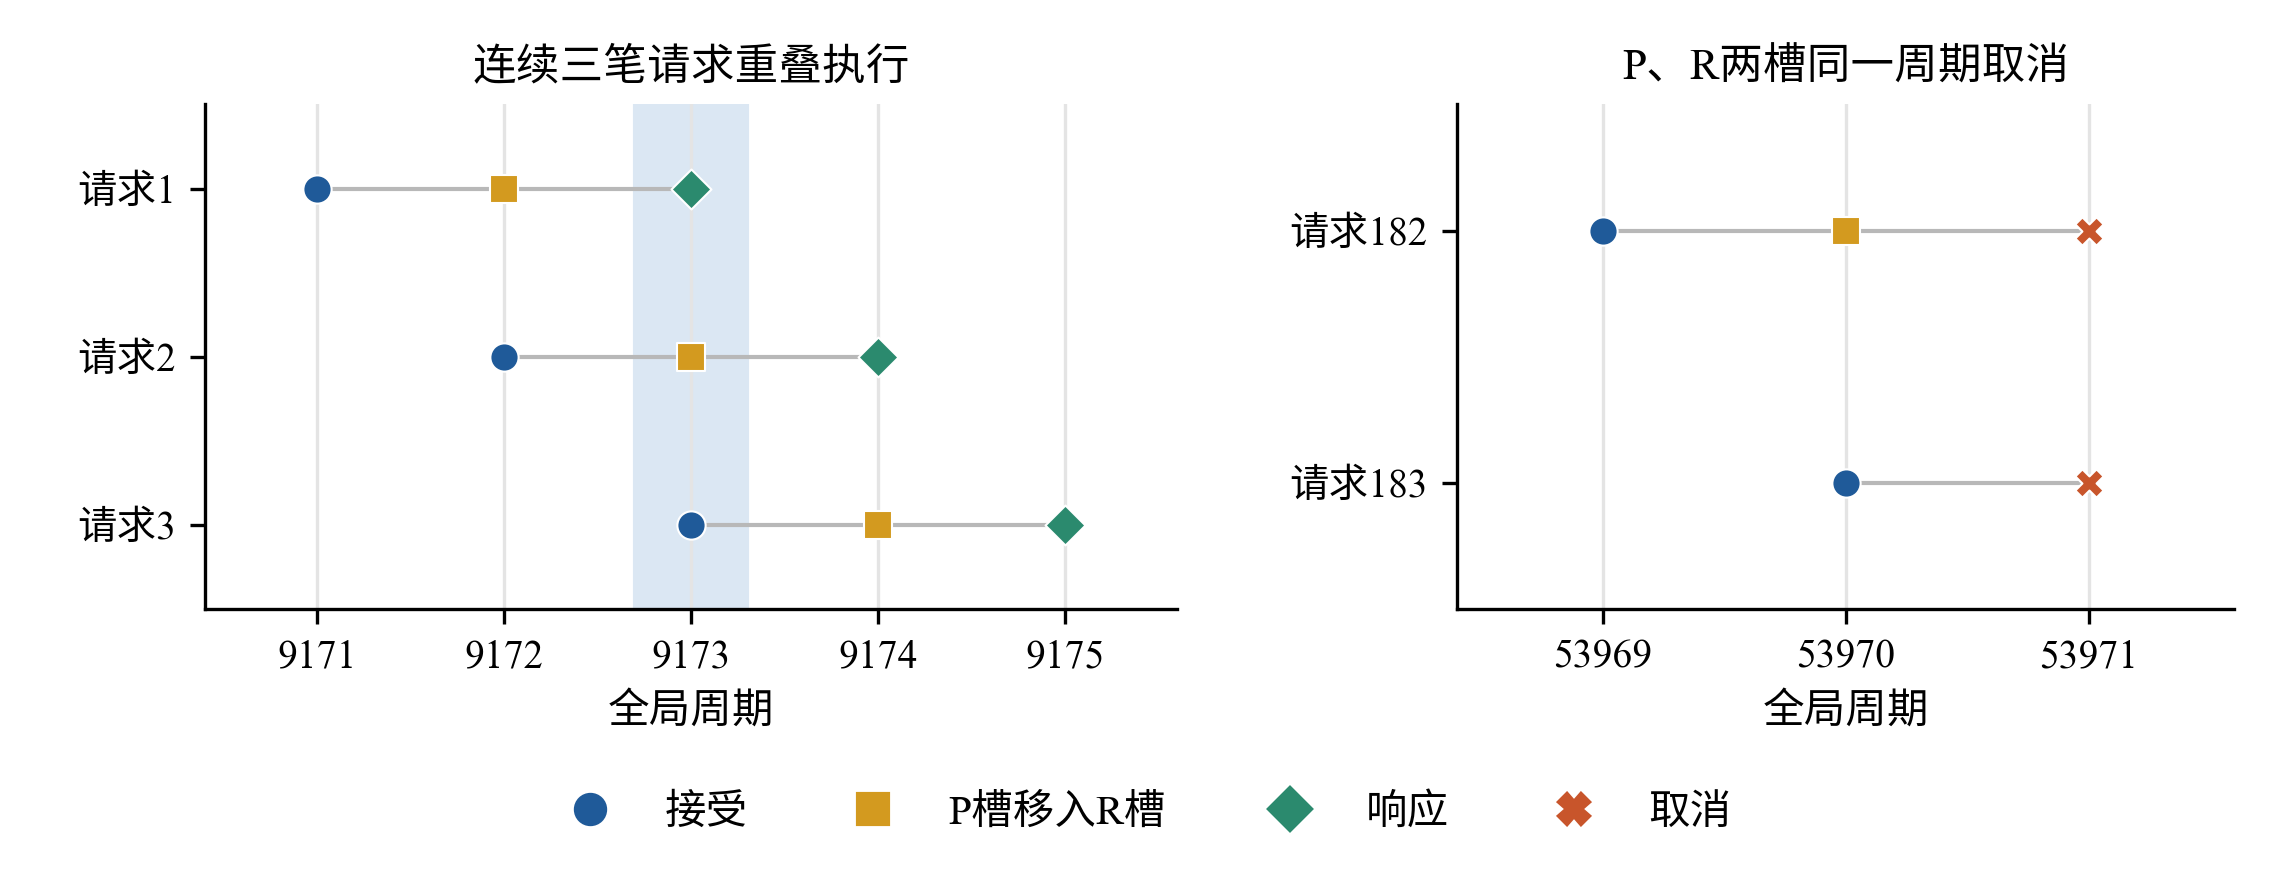
\includegraphics[width=0.92\linewidth]{fig03_control_events.png}
\caption{控制诊断日志中的流水重叠与两槽取消}\label{fig:control}
\end{figure}

原始日志为\ev{evidence/C02__run.log.gz}，图中事件对应的原始行见\ev{evidence/C02-selected-events.txt}，运行结果与统计为\ev{evidence/C01__result.json}和\ev{evidence/C03__functional-result.json}。

\subsection{全核波形}\label{sec:s3-wave}

2026年11月5日用受测版本的RTL单独构建了可输出FST波形的EMU，运行functional-2并开启DiffTest，程序到达GOOD TRAP、以状态0退出。波形中选取正数点积（两源低8字节为1至8，结果204）这一笔事务，按ROB编号39、物理目的103、PC \texttt{0x80001b8c}和机器字\texttt{0x0294050b}关联输入、响应与提交，如表\ref{tab:wave}。

\begin{table}[!htbp]\centering\small
\caption{正数点积事务的波形坐标}\label{tab:wave}
\begin{tabular}{lrr}
\toprule
事件 & 波形坐标 & 观察器周期\\
\midrule
输入有效 & 678694 & ---\\
接受 & 678696 & 339296\\
输出有效 & 678698 & ---\\
响应握手 & 678700 & 339298\\
ROB提交 & 678706 & 339301\\
DiffTest提交观察 & 678710 & ---\\
\bottomrule
\end{tabular}
\par\smallskip
{\footnotesize 注：波形每个周期占2个坐标单位；坐标除以2后与观察器周期相差固定的52个周期。}
\end{table}

\begin{figure}[!htbp]\centering
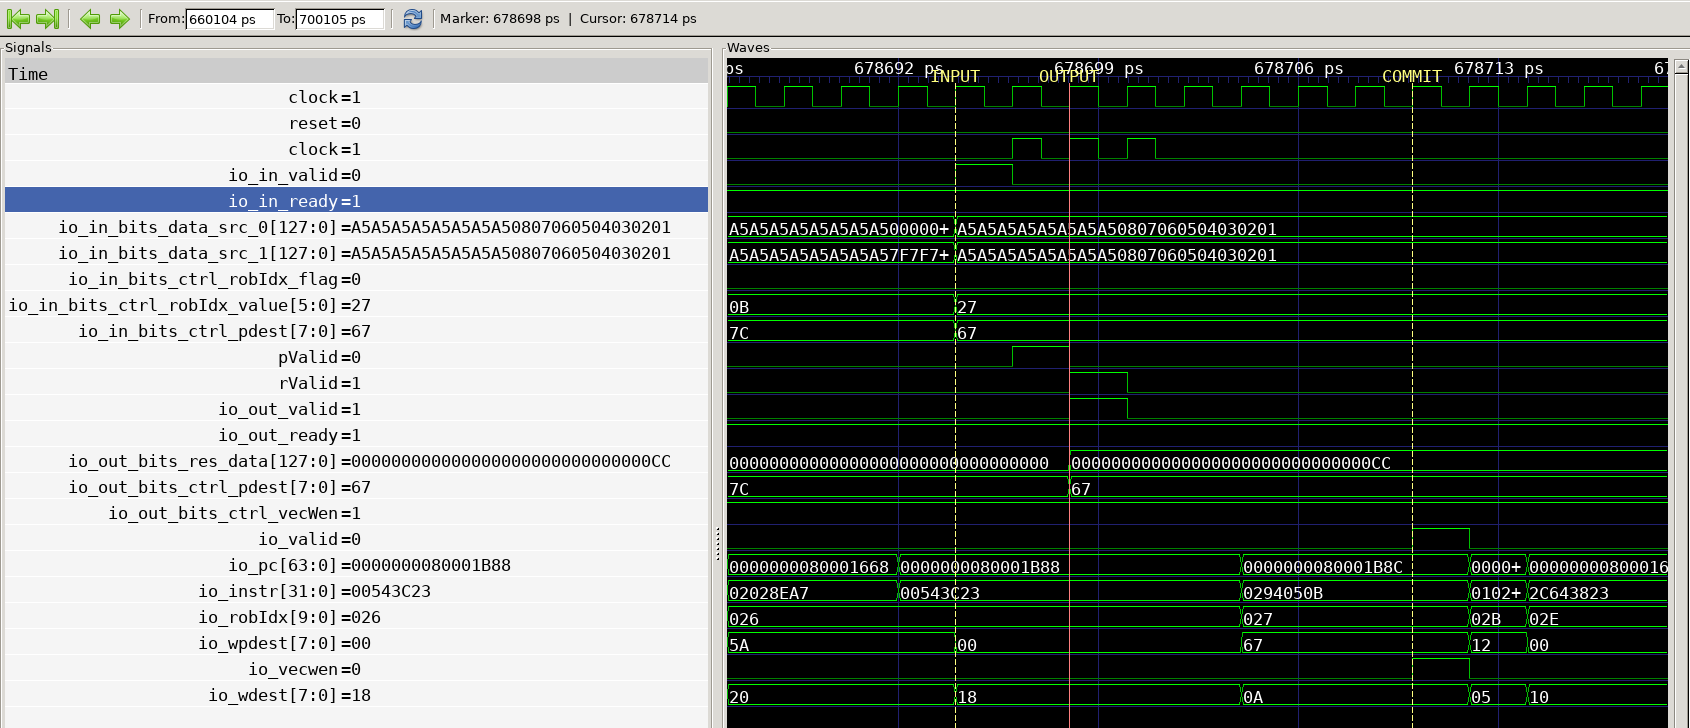
\includegraphics[width=\linewidth,height=8cm,keepaspectratio]{S3-WAVE-02.png}
\caption{结果有效与响应握手：结果204，高96位为零}\label{fig:wave}
\end{figure}

运行命令、信号清单、采样值与核对结果保存在\ev{evidence/W01_vdot-wave-20261105/}，三幅GTKWave截图为\ev{evidence/G01_report-screenshots/S3-WAVE-01.png}至\ev{S3-WAVE-03.png}。同一目录还有原始波形文件\ev{vdot-positive.fst}（159\,MB）、GTKWave视图文件\ev{vdot-positive.gtkw}和运行日志\ev{run.log}；用GTKWave打开波形并载入视图文件，即可看到截图中的信号。这次运行共执行607,250条指令、775,767个周期，与10月27日干净环境复现中functional-2的原运行完全相同。

\subsection{RVV基线与测量方法}

赛题要求的RVV基线用标准向量指令实现相同的8项有符号点积：先用\texttt{vwmul.vv}得到16位乘积，再切换到e16/m1/VL8，以\texttt{vwredsum.vs}归约得到完整整数和，高96位保持为零。基线程序源码见\ev{evidence/B30_rvv-baseline/}。

周期由程序读取cycle和instret计数器得到，读数前后用fence隔开。观察器记录了四条CSR读取指令进入ROB、采样和退休的时刻，确认cycle差等于全核采样周期差、instret差等于窗口内退休的指令数；测量规范见\ev{evidence/T13__measurement-contract-README.md}。每个场景使用3组数据，每组取4个正式窗口，首次执行和预热窗口单独记录，不计入均值。

\subsection{微基准}\label{sec:s3-micro}

VDot与RVV路径在同一程序镜像中运行，输入、循环次数和计时边界相同。结果见表\ref{tab:micro}和图\ref{fig:micro}，全部窗口数据在\ev{data/微基准全部窗口.csv}，原始窗口文件为\ev{evidence/B00__window-result.json}至\ev{B23__window-result.json}（2026年10月25日）。

\begin{table}[!htbp]\centering\small
\caption{四类微基准（每种实现12个正式窗口的平均DUT周期）}\label{tab:micro}
\begin{tabular}{lrrrr}
\toprule
场景 & VDot & RVV & 加速比 & VDot窗口范围\\
\midrule
单次点积 & 71 & 85.25 & 1.2007$\times$ & 71--71\\
依赖链（256次） & 1857 & 5440.5 & 2.9297$\times$ & 1857--1857\\
四路独立批量（128次） & 221 & 678 & 3.0679$\times$ & 221--221\\
加载、计算、存储流（64次） & 1127.5 & 1133 & 1.0049$\times$ & 1119--1131\\
\bottomrule
\end{tabular}
\end{table}

\begin{figure}[!htbp]\centering
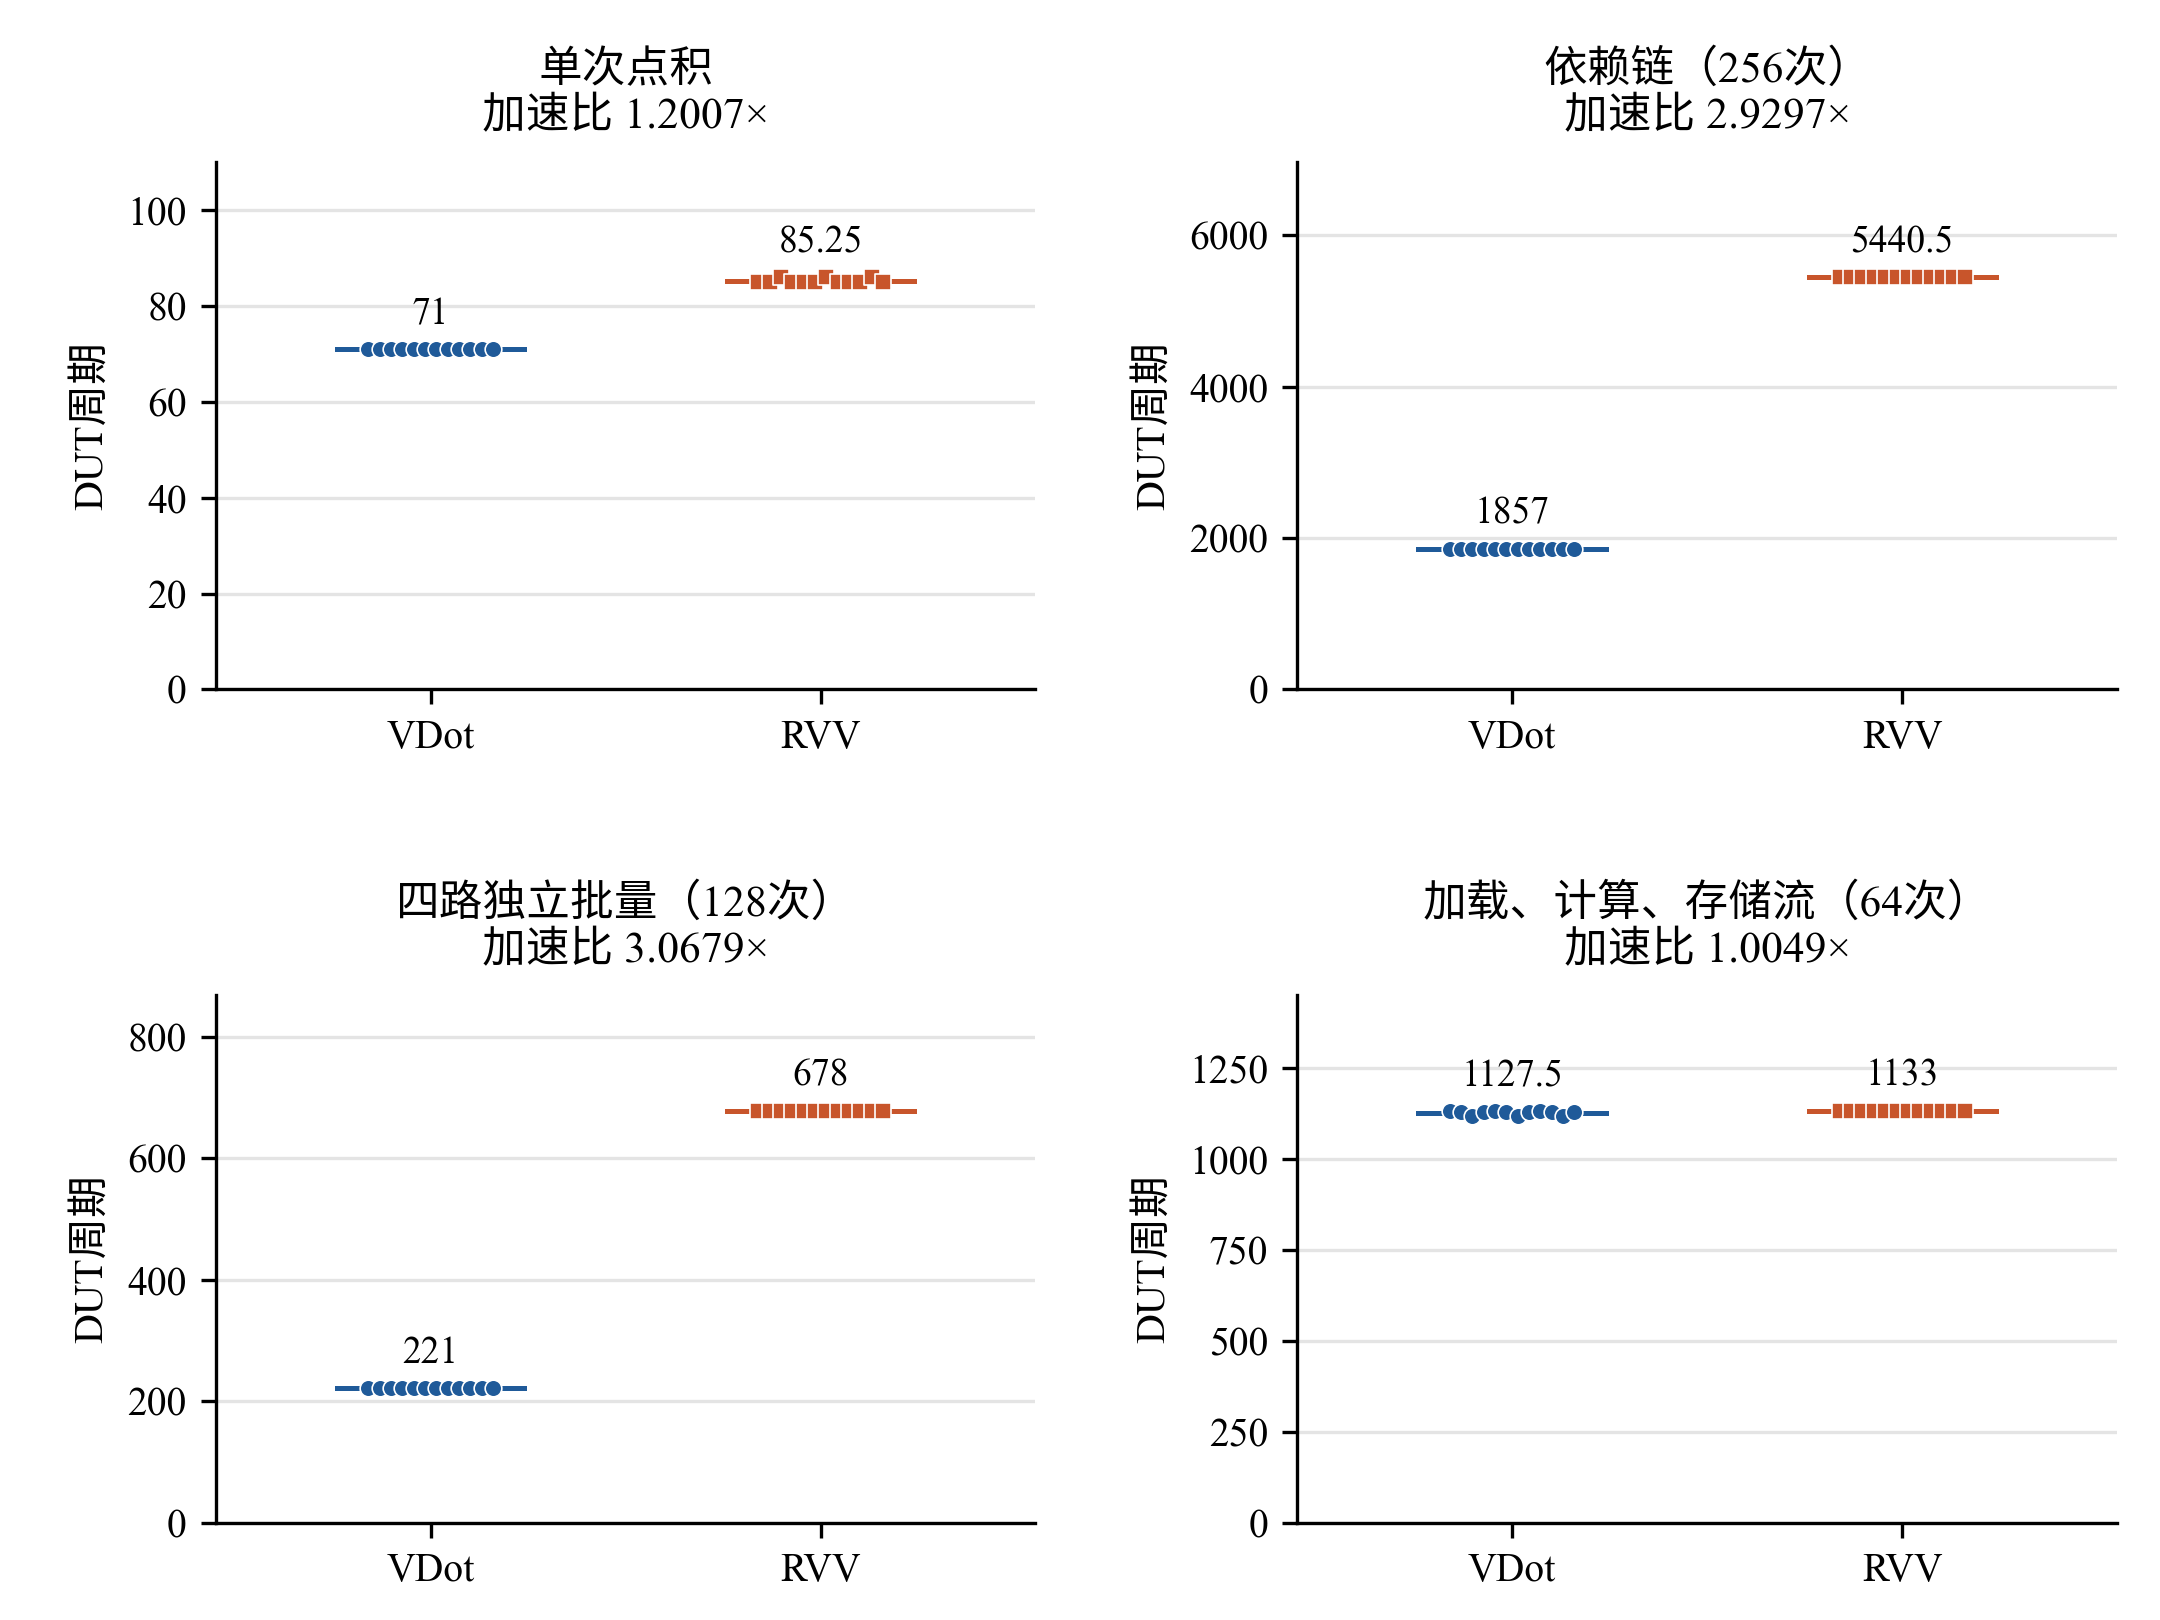
\includegraphics[width=0.88\linewidth]{fig01_microbench.png}
\caption{四类微基准的全部正式窗口（点为单个窗口，横线为均值）}\label{fig:micro}
\end{figure}

独立批量的加速主要来自两槽设计：同一镜像中，上一版单笔在途设计需要362.5周期，两槽设计为221周期，减少39.0\%（\ev{evidence/O01__two-slot-vs-single-inflight.md}）。加入DIV取消修复前后，同一输入的96对正式窗口周期完全相同（\ev{evidence/O02__microbench-div-cancel-result.md}）。

\subsection{8×32 GEMV调用}\label{sec:s3-c8}

C8软件包提供普通C接口\texttt{xs\_c8\_gemv\_8x32}，输入为288字节的$A[8][32]$与$x[32]$，输出8个16字节结果槽。三种实现在同一EMU上运行，计时覆盖一次完整函数调用（含C调用开销），结果见表\ref{tab:c8}和图\ref{fig:c8}。

\begin{table}[!htbp]\centering\small
\caption{8×32 GEMV调用（每种实现12个正式窗口）}\label{tab:c8}
\begin{tabular}{lrrr}
\toprule
实现 & 平均周期 & 范围 & 每窗口指令数\\
\midrule
首段初始化版本（VDot） & 282.25 & 282--283 & 182\\
C8配置复用版本（VDot） & 273 & 273--273 & 175\\
较快的RVV实现 & 299 & 296--302 & 123\\
\bottomrule
\end{tabular}
\end{table}

\begin{figure}[!htbp]\centering
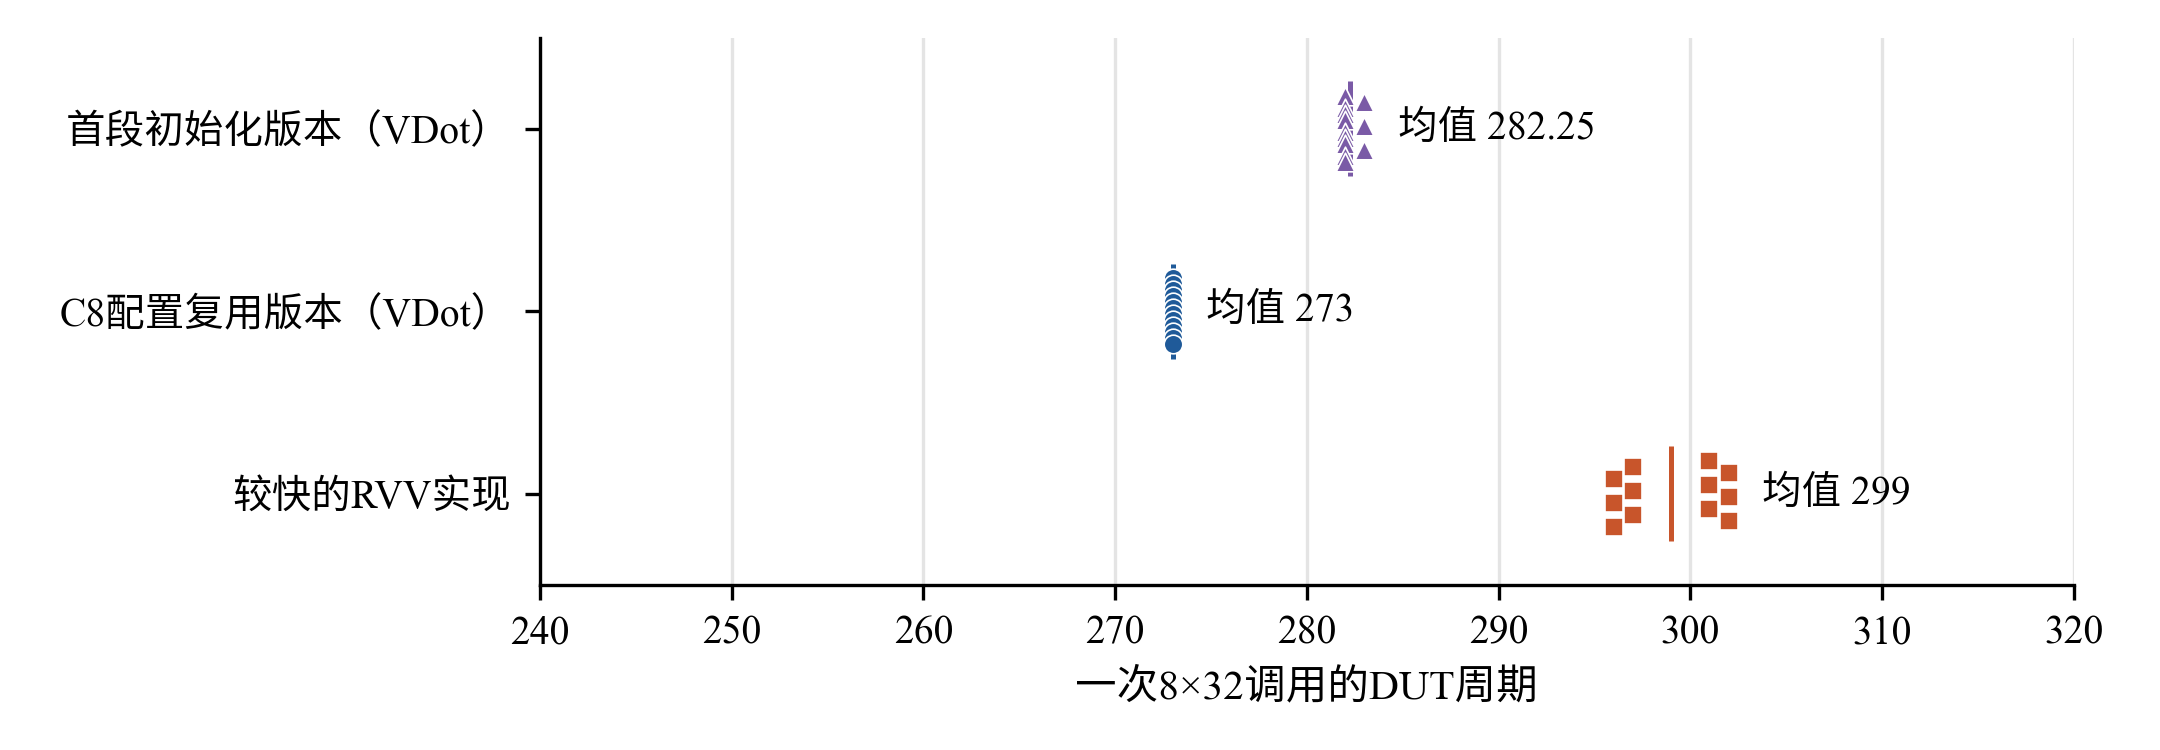
\includegraphics[width=0.88\linewidth]{fig02_c8.png}
\caption{8×32 GEMV调用的全部正式窗口}\label{fig:c8}
\end{figure}

C8比较快的RVV实现快$299/273=1.095$倍，比首段初始化版本少用3.3\%的周期；RVV实现的指令更少，周期却更多。测量矩阵为\ev{evidence/P08__results.json}，六份原始标准输出为\ev{evidence/L0__stdout.log}至\ev{Q2__stdout.log}，参与比较的36个窗口列在\ev{data/C8最终尺寸正式窗口.csv}。

功能方面，C8的16个公共函数在48个不同用例上完成普通C调用测试，两次运行共96次调用全部正确（\ev{evidence/P01__results.json}）。封装成静态库后，最终程序与测试时的31,440字节BIN逐字节一致（\ev{evidence/P10__c8-relink-equivalence.md}），接口与验收结果见\ev{evidence/P11__c8-package-result.md}。

\subsection{完整前向计算}\label{sec:s3-forward}

量化GEMV内核接入一个六层Transformer（模型维度288，前馈维度768，词表32,000），在香山仿真模型上执行token=1、position=0的一次完整前向。FR使用标准RVV内核，TA使用VDot内核；两路都通过DiffTest以及3,691,424字节的完整状态比较，TA的独立重放得到完全相同的结果和计数。仿真环境的硬件提交为\texttt{34bae6d4}。

\begin{table}[!htbp]\centering\small
\caption{完整前向的计数窗口（各一次）}\label{tab:forward}
\begin{tabular}{lrrr}
\toprule
实现 & 周期 & 退休指令 & 执行的vdot\\
\midrule
FR：标准RVV & 20,258,039 & 7,502,872 & 0\\
TA：VDot & 19,774,245 & 10,122,100 & 1,949,184\\
TA重放 & 19,774,245 & 10,122,100 & 1,949,184\\
\bottomrule
\end{tabular}
\end{table}

TA比FR少用2.4\%的周期。TA窗口中的1,949,184条vdot有1,949,182条在2个周期内响应，其余2条为3个周期。各运行的四条CSR读取都通过了采样与退休时刻核对。汇总见\ev{evidence/M01_forward-fr-ta/analysis/target-summary.json}，逐次结果在同目录\ev{audit/target/}。

2026年11月6日，在同一模型上另做了三种标准RVV实现的对比。三种实现共用一个ELF（SHA-256前缀\texttt{be6c3ead424d}），都通过了DiffTest与完整状态比较：

\begin{table}[!htbp]\centering\small
\caption{三种RVV实现的完整前向窗口（各一次）}\label{tab:rvv3}
\begin{tabular}{lrrr}
\toprule
实现 & 周期 & 退休指令 & 相对FR周期减少\\
\midrule
FR & 22,244,288 & 7,502,886 & ---\\
GS32 & 19,996,570 & 4,828,788 & 10.10\%\\
paired16 & 17,382,632 & 5,175,371 & 21.86\%\\
\bottomrule
\end{tabular}
\end{table}

这一组重新编译了包含三种路径的共同程序，程序布局与表\ref{tab:forward}不同，因此两表的FR周期不同，两组数据只在组内比较。原始结果为\ev{evidence/M02_forward-rvv3/target-v1/raw.zip}，说明见同目录\ev{REFERENCE.md}。

\subsection{综合面积与时序}\label{sec:s3-cost}

受测版本的独立VDot FU和完整VFEX4父级（含VDot、DIV/SQRT和共享控制）按4\,ns目标综合，再做4\,ns、5\,fF的布局前setup检查（2026年11月8日）。工艺库为Nangate45 Typical（1.10\,V、25\,°C），工具为Yosys 0.9、ABC 1.01和OpenSTA 2.0.17。

\begin{table}[!htbp]\centering\small
\caption{4 ns综合面积与setup检查}\label{tab:sta}
\begin{tabular}{lrr}
\toprule
指标 & 独立VDot FU & 完整VFEX4父级\\
\midrule
标准单元面积（$\mu\mathrm{m}^2$） & 17112.578 & 284562.278\\
寄存器到寄存器路径裕量（ns） & $+2.722349$ & $+0.436214$\\
全局最差setup裕量（ns） & $+2.601416$ & $+0.422254$\\
路径类别 & 5类全部满足 & 9类全部满足\\
\bottomrule
\end{tabular}
\end{table}

FU面积约占父级的6.0\%，父级的最差路径不在VDot上。图\ref{fig:sta}为全部14类路径的裕量。约束、路径报告和输入版本在\ev{evidence/K01_nangate45-4ns-20261108/}，汇总为其中的\ev{RESULT.json}。同一父级此前按1\,ns约束综合时寄存器到寄存器裕量为$-2.34$\,ns（\ev{evidence/T04__summary.json}至\ev{T06__result.json}，2026年10月25日），除法等原有逻辑在这一频率附近无法闭合，这是成本比较统一采用4\,ns的原因。以上为局部模块的布局前分析，不含布线后时序与功耗。

\begin{figure}[!htbp]\centering
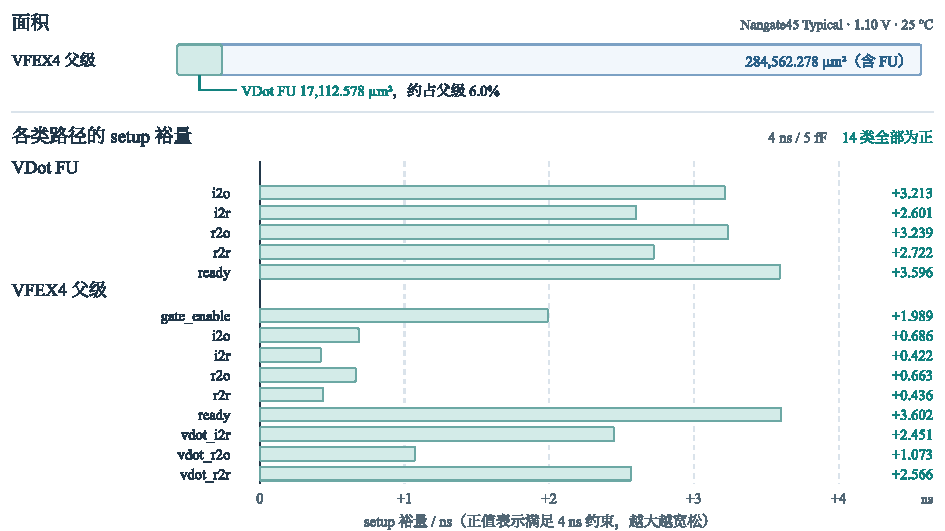
\includegraphics[width=\linewidth,height=9cm,keepaspectratio]{fig04_sta_4ns.pdf}
\caption{Nangate45模块面积与4 ns／5 fF setup裕量}\label{fig:sta}
\end{figure}

一拍运算的SP1方案与稳定版在相同工具、工艺库和约束下对比如表\ref{tab:sp1}（SP1提交\texttt{ffb52e45}）。SP1使依赖链周期减少13.8\%，其余场景基本不变，FU面积增加6.1\%，VDot输入到寄存器路径的裕量减少约0.7\,ns；最终提交采用稳定版。数据在\ev{evidence/K02_sp1-4ns-comparison-20261108/}。

\begin{table}[!htbp]\centering\small
\caption{稳定版与SP1}\label{tab:sp1}
\begin{tabular}{lrr}
\toprule
指标 & 稳定版 & SP1\\
\midrule
依赖链周期（256次） & 1857 & 1601.25\\
单次点积周期 & 71 & 70\\
四路独立批量周期（128次） & 221 & 221\\
C8调用周期 & 273 & 272\\
独立FU面积（$\mu\mathrm{m}^2$） & 17112.578 & 18156.628\\
独立FU最差setup裕量（ns） & $+2.601416$ & $+1.951567$\\
父级VDot输入到寄存器裕量（ns） & $+2.450936$ & $+1.742610$\\
\bottomrule
\end{tabular}
\end{table}

团队于2026年10月28日还用同一份RTL（源码提交\texttt{e1815c07}，两拍运算的两槽实现）分别以Nangate45和ASAP7综合，ABC目标与STA周期均为1\,ns。换用ASAP7后FU和父级面积分别减少92.7\%和93.2\%；父级最差裕量为$-0.65$\,ns，放宽到2\,ns后全部满足。数据在\ev{evidence/K03_asap7-reference-20261108/}，与表\ref{tab:sta}的条件不同，只在两库之间比较。

\section{复核方法}

{\raggedright
\begin{itemize}
\item \textbf{文件完整性}：在本材料根目录执行\texttt{python tools/verify\_package.py}，核对全部文件的大小与SHA-256。
\item \textbf{原始日志}：\texttt{python reference/submission/logs/read\_log.py list --contains rtl-datapath}按路径查找，\texttt{show}输出单个日志，\texttt{verify}校验7卷归档。
\item \textbf{重新运行}：完整代码在\repo{\Rel}{submission/REPRODUCE.md}{发布提交的复现说明}中给出构建与运行步骤，主机检查可用\texttt{bash submission/reproduce.sh check}一次执行。环境要求见\ev{reference/submission/docs/ENVIRONMENT.md}。
\item \textbf{数据图}：\texttt{python tools/draw\_figures.py}从\ev{data/}重新生成图\ref{fig:control}、图\ref{fig:micro}和图\ref{fig:c8}。
\end{itemize}\par}

\appendix
\section{名称对照}

原始记录保留了开发时的内部名称，与报告和本文名称的对应关系如表\ref{tab:names}。

\begin{table}[!htbp]\centering\small
\caption{本文名称与原始记录中的名称}\label{tab:names}
\begin{tabular}{p{0.34\linewidth}p{0.56\linewidth}}
\toprule
本文名称 & 原始记录中的名称\\
\midrule
受测版本、稳定版 & \texttt{0f}、firstdot V2 0f\\
两槽设计 & O2、\texttt{VDOT\_O2\_ELASTIC=1}\\
上一版单笔在途设计 & O1\\
首段初始化版本 & firstdot V2\\
C8配置复用版本 & C8、config-reuse\\
干净环境复现构建 & clean-02\\
控制诊断 & control diagnostic、T13/O2 observer\\
完整前向 FR／TA & first-token forward，FR、TA\\
\bottomrule
\end{tabular}
\end{table}

\section{原始记录索引}

{\small\setlength{\tabcolsep}{4pt}
\begin{longtable}{>{\raggedright\arraybackslash}p{0.42\linewidth}>{\raggedright\arraybackslash}p{0.50\linewidth}}
\caption{evidence目录}\label{tab:evidence}\\
\toprule
文件或目录 & 内容\\
\midrule\endfirsthead
\caption[]{evidence目录（续）}\\
\toprule
文件或目录 & 内容\\
\midrule\endhead
\ev{S01}～\ev{S07} & 第一阶段10月9日运行：验收标记、运行摘要、提交事件、工具版本、首次与成功运行日志\\
\ev{S10_hello-20261025/} & 第一阶段10月25日复核：两次运行记录与FST/VCD波形\\
\ev{S20_build-logs-20261009/} & 第一阶段10月9日的NEMU、EMU与测试程序构建日志\\
\ev{D01}～\ev{D03} & 测试数据定义、定向向量、状态向量\\
\ev{A01}～\ev{A04} & 算术RTL测试结果、源文件哈希、错误注入\\
\ev{F01}～\ev{F04} & 全核功能分片、高位负控、最终组合验收\\
\ev{F10_basic-test-logs/} & 基础测试的两份完整运行日志\\
\ev{G01_report-screenshots/} & 基础测试日志、负控与波形截图\\
\ev{R01}～\ev{R05} & 11月8日在发布提交上的检查日志\\
\ev{N01}～\ev{N07} & 11月8日早些时候的同类检查与软件库链接检查\\
\ev{N10_nemu-patch/} & NEMU vdot补丁\\
\ev{C01}～\ev{C03} & 控制诊断运行结果、原始日志、功能统计\\
\ev{W01_vdot-wave-20261105/} & 全核波形的运行命令、信号、采样、核对结果与波形文件\\
\ev{B00}～\ev{B23} & 微基准原始窗口\\
\ev{B30_rvv-baseline/} & RVV基线程序源码\\
\ev{T04}～\ev{T06} & 受测版本父级的1\,ns综合与STA记录\\
\ev{T01}～\ev{T03} & 早期版本的成本与STA记录\\
\ev{T13__measurement-contract-README.md} & 周期测量规范\\
\ev{O01}，\ev{O02} & 两槽与单笔在途设计对比、DIV取消修复前后对比\\
\ev{P01}～\ev{P11}，\ev{L0}～\ev{Q2} & C8功能、测量矩阵、原始输出与封装等价\\
\ev{M01_forward-fr-ta/}，\ev{M02_forward-rvv3/} & 完整前向的运行结果\\
\ev{K01}～\ev{K03} & 4\,ns综合、SP1对比、双工艺库参考\\
\ev{H01}，\ev{H02}，\ev{V01}，\ev{V02} & 生产源码固定清单与最终版本身份\\
\bottomrule
\end{longtable}}

每个文件的原路径、来源提交、字节数和SHA-256见\ev{data/精选证据索引.tsv}；日志归档的全部成员见\ev{data/完整原始日志索引.tsv}。

\end{document}
